\pagebreak
  \chapter{Annexes}
  \pagebreak

  \section{Pattern Map} \label{anex:pat:map}
    \begin{figure}[ht!]
        \includegraphics[width=1\linewidth]{./figures/patterns.png}
    \end{figure}
\pagebreak
  \section{Concepts Grouping} \label{anex:pat:group}
    \begin{figure}[ht!]
        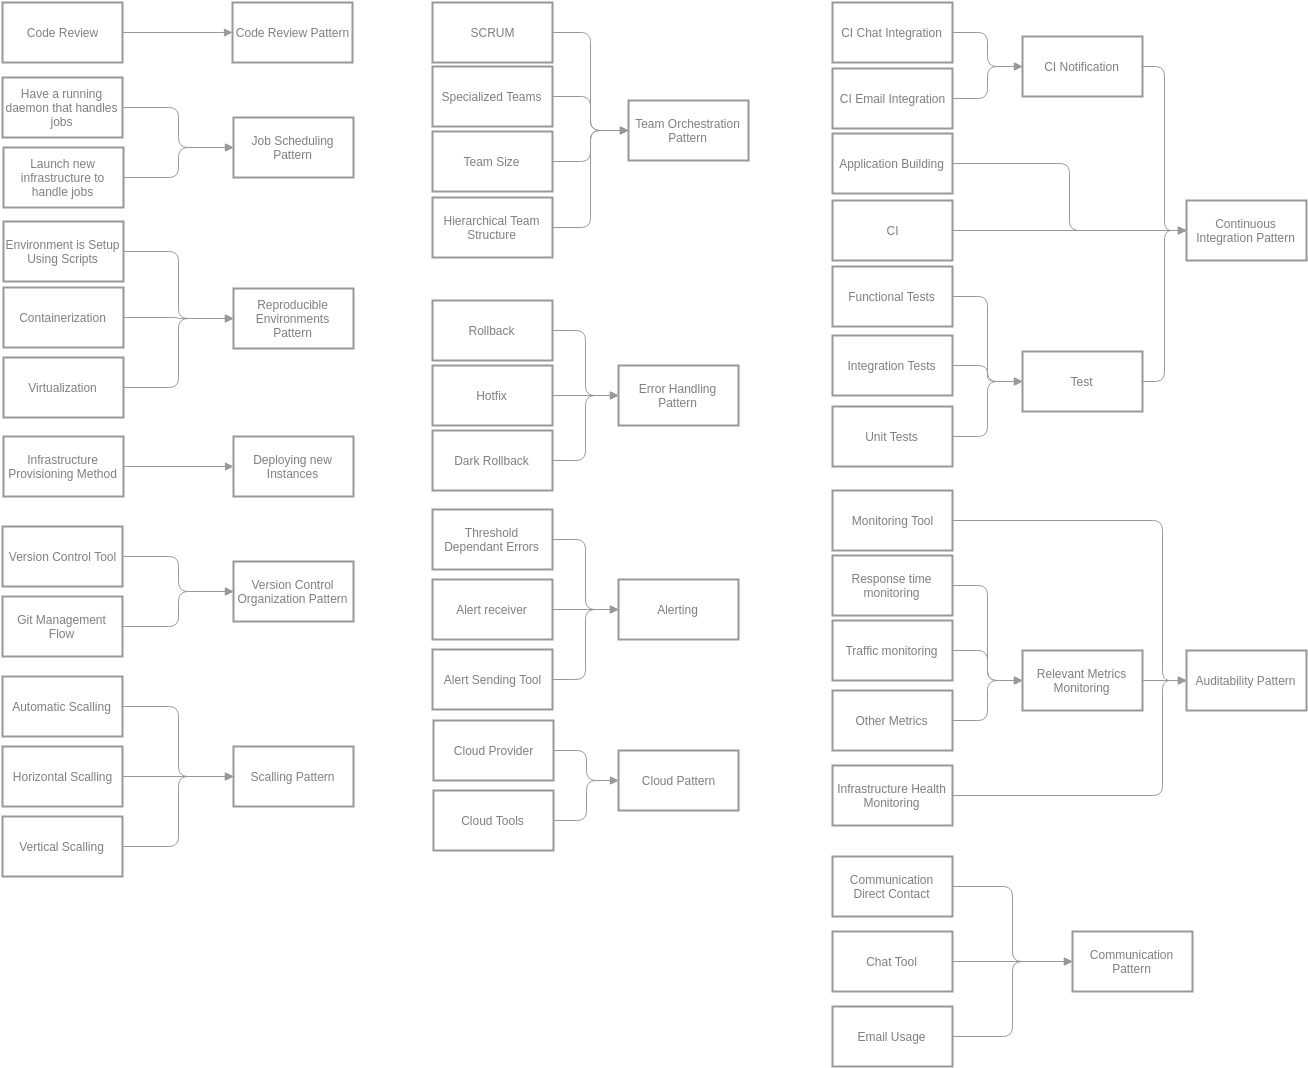
\includegraphics[width=1\linewidth]{./figures/concepts.png}
    \end{figure}
\pagebreak
\begin{landscape}
    \begin{figure}[ht!]
      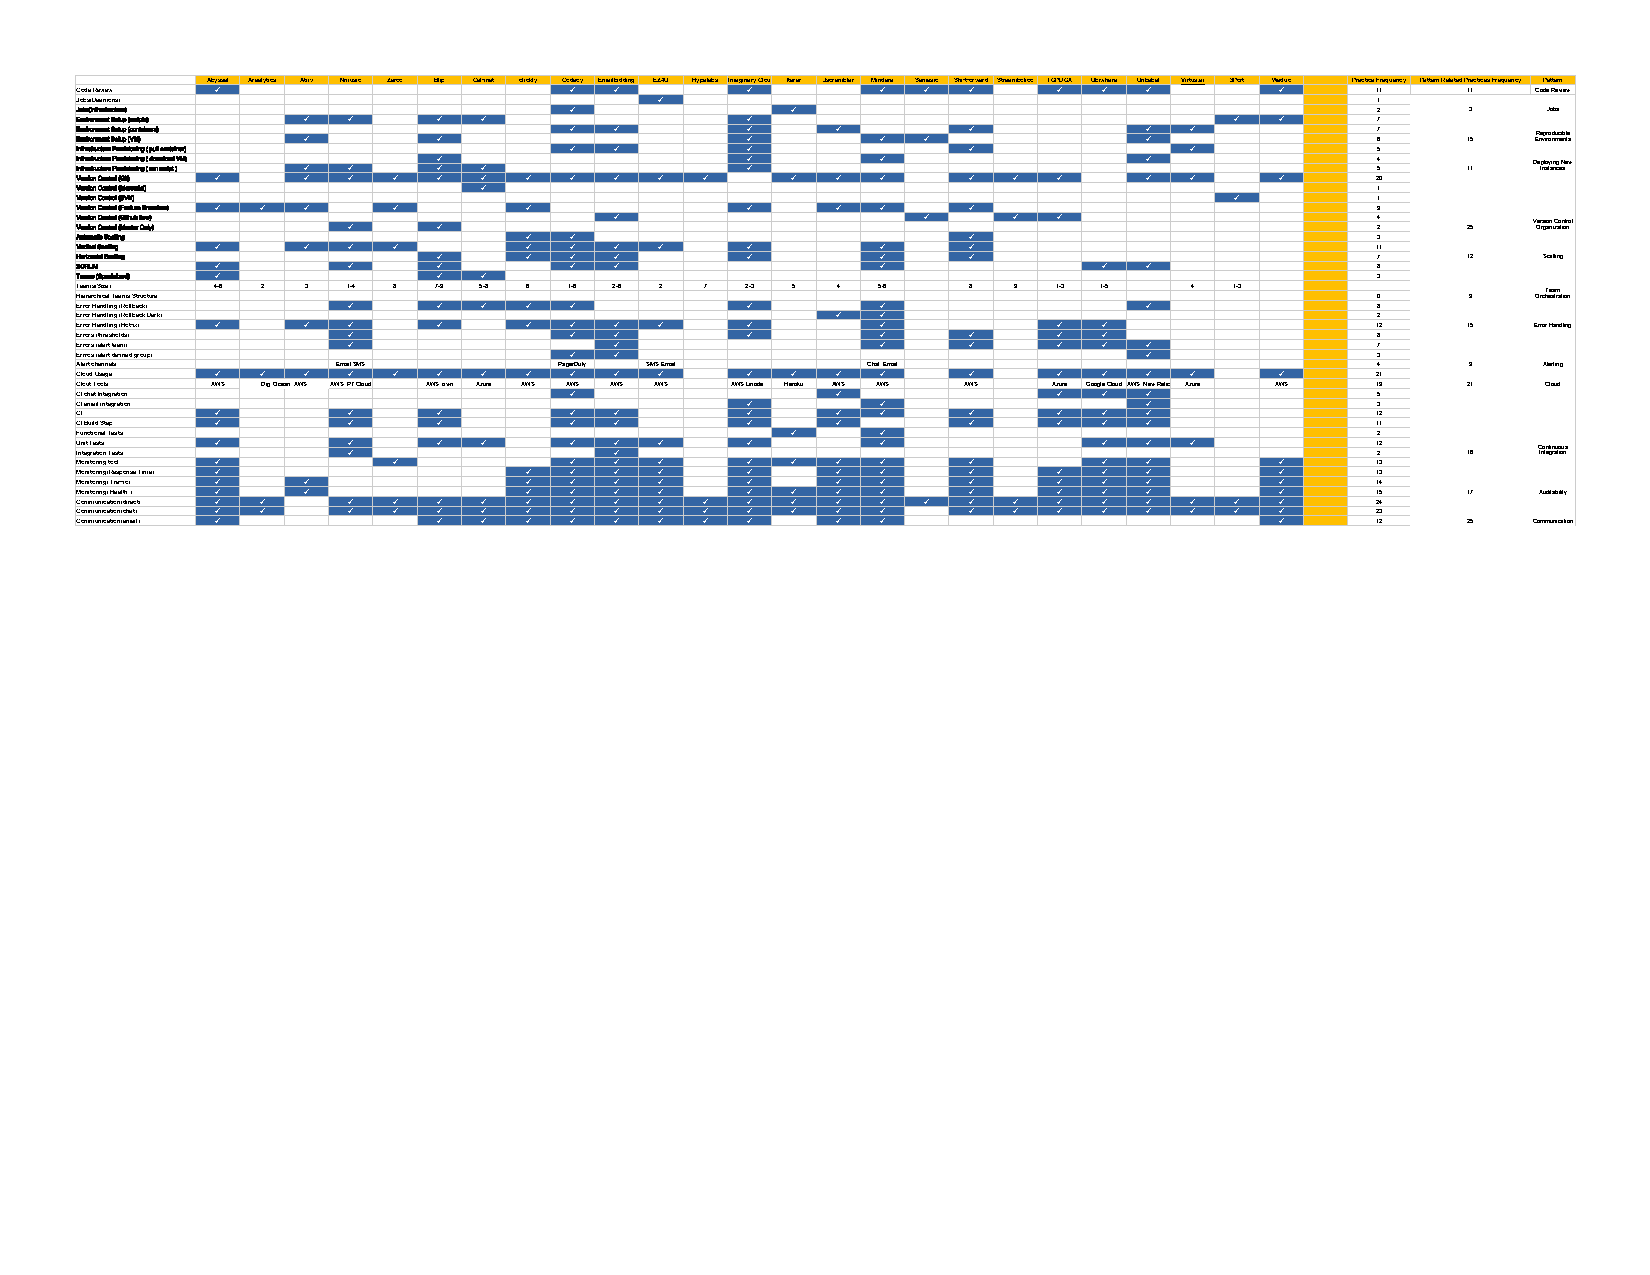
\includegraphics[height=0.8\linewidth]{patterns_stats.pdf}
      \caption{Interview practices frequency extraction.}
      \label{anex:pat:freq}
    \end{figure}
\end{landscape}

\pagebreak

  \section{Interview Guide} \label{anex:interview}
    \subsection*{Product}
        \begin{itemize}
            \item What type of product do you develop ?
            \item What is the scale of that product ? Number of countries, number of users ?
            \item Do you have some kind of SLA or some requirements that impacts your work ?
    \end{itemize}
    \subsection*{Teams}
        \begin{itemize}
            \item How many teams do you have ?
            \item What is the size of each team ?
            \item Are teams specicalized or do they have multiple specializations working together ?
            \item Do teams interact with each other ?
            \item How are teams seen from an external perspective ? Are they autonomous?
            \item How do you manage your workload ? Do you use SCRUM,Kanban or other ?
            \item How do team members communicate among themselves.
    \end{itemize}
    \subsection*{Pipeline}
  	    \begin{itemize}
            \item How long does your code take to go from idea to production ?
            \item What are the states that you code goes through before reaching a production environment
            \item What triggers the transition between states ?
            \item What kind of tests do you develop? Which teams are involved in that process ? When do they run?
            \item What happens in each of the pipeline states ?
            \item In each state, which teams intervene and what do they do?
            \item What processes did you automate ? Did you choose to not automate some state ? If so, why?
            \item How do you handle your deployment process ? Which tools do you use ? Do you use containers or VMs ?
    \end{itemize}
    \subsection*{Infrastructure Management}
        \begin{itemize}
            \item How do you scale ? Horizontally or vertically?
            \item Does scalling happen automtatically ?
            \item What can make infrastructure scale up/down ?
            \item How is infrastructure increased ?
            \item How do you lift new instances of your infrastructure? Is it automatic?
    \end{itemize}
    \subsection*{Monitoring \& Error Handling}
  	    \begin{itemize}
            \item What metrics do you collect from running servers ?
            \item What do you see as errors ?
            \item What process do you follow to solve errors after they are detected ?
            \item When errors are detected, who is notified ? How is the notification sent ?
            \item If errors are detected before the software reaches production, what do you do ?
        \end{itemize}
\pagebreak

  \section{Companie Interviews Report} \label{anexes:interviews}
    \begin{companyreport}{Abyssal}
        \product
        Abyssal is a startup company focused on developing Subsea Navigation Systems for Remotely Operated Vehicles (ROVs) operating since 1 de Fevereiro 2012.\\
        Their goal is to facilitate the access to these locations by developing intuitive and precise software solutions to the major problems affecting ROV piloting and supervision: poor navigation, reduced visibility and lack of spatial\\ awareness.\\
        The current solutions has two major modules. One that renders the underwater obstacles in the live video feed from the ROVs and a web one that handles the transmission of data from the rig/ship to shore.
        \teams
        Teams at abyssal are mainly divided by area of specialization and have between 6-4 people. Nevertheless, roles inside each team sometimes change(see below). Teams communicate both directly and through Slack. Confluence is used as as a collaboration platform.\\
        In order to manage the project, Abyssal uses SCRUM.
        \development
        The development process at abyssal focus on three languages : C++. C\# and Python. In order to manage their code, Abyssal uses Git with feature branches.\\
        Unitary tests are developed by the development team, manual tests are performed by one member of the development team (the role is changed every sprint). This unitary tests are then used in the Continuous Integration phase.\\
        A code review process was also implemented. Every feature is analysed by one member of the development team. This member must not be the same one that did the feature.\\
        Continuous Integration is managed by Team City. Team City is responsible for creating a build and running the existent tests.
        \operations
        Abyssal uses AWS services in order to manage their infrastructure. Due to well defined upper and lower bounds for users numbers and load scaling is done only manually at Abyssal.\\
        Deployments and upgrades are mainly managed  manually except for the Virtual Reality where a tool assists the the deployment process.\\
        Logs are stored in the running instances and retrieved manually when needed.\\
        Monitoring relies on AWS services and the main metrics monitored are server load and and disk space.\\
        When errors are detected, Abyssal usually solves them by issuing a hotfix.
        \reportend
    \end{companyreport}

    \begin{companyreport}{arealytic}
      \product
      arealytic is a young company ( 5 month old in the time this interview was conducted) that wants to transform IP  and other types of cameras into analytics tools. In order to do this, arealytic developed a web platform that analyzes camera footage and tracks user movements throughout a store as well as interactions with displayed products.\\
      \teams
      The arealytic team had at the time two members. Both worked in all aspects of the product and communicated either directly or by using Slack.\\
      \development
      The development process at abyssal focus on three languages : PHP, Javascript and Python. In order to manage their code, arealytic uses Git with feature branches.\\
      \reportend
    \end{companyreport}

    \begin{companyreport}{Atiiv}
      \product
      Atiiv is a company that develops a web platform for Personal Trainers to monitor, register and prescribe training plans to it's clients.\\
      At the time of the interview the company was roughly 1.5 years old and had 4 collaborators.\\
      \teams
      Teams at Atiiv have 3 people and communicate  using several a chat tool.
      \development
      The development process at Atiiv focus on two languages: PHP and Javascritp . In order to manage their code, Atiiv uses Git  with feature branches. \\
      Unitary tests are developed by the development team, manual tests are also performed by the development team.
      \operations
      Atiiv uses Digital Ocean and AWS services in order to manage their infrastructure.  \\
      Deployments and upgrades are managed by Laravel Forge (a PaaS service). \\
      Monitoring relies on New Relic services and some of the metrics monitored are the server state and load. \\
      When errors are detected, Atiiv usually solves them by doing a hotfix.
      \reportend
    \end{companyreport}

    \begin{companyreport}{NMusic}
      \product
      NMusic is a portuguese startup that develops a platform that allows other businesses to stream and synchronize music.
      \teams
      Teams at NMusic are mainly divided by speciality and have between 1-4 people. Teams communicate  both directly for doubts and discussions and using Slack to share files and links.
      \development
      In order to manage their code, NMusic uses Git with only a master branch.  \\
      Unit tests are developed by the Development team and manual tests are performed by a QA team. \\
      Continuous Integration is managed by Jenkins and its main objective is to create a nightly build . This tool is  responsible for creating a build and running the existing tests.
      \operations
      NMusic uses AWS and PT Cloud services in order to manage their infrastructure.\\
      Deployments and upgrades managed by Capistrano .\\
      Monitoring relies on Zabbix. If errors are detected depending on their severity different approaches can be adopted. If an error is not critical, an internal interface will be updated, if an error is bad but still not critical, an email is sent. In a case where an error is considered critical there are two developers that are notified by SMS. Some common solutions at NMusic can be issuing a hotfix or deploying the previous version.
      \reportend
    \end{companyreport}

    \begin{companyreport}{Zarco}
      \product
      Zarco is a mobile app that aims to link travelers with traveling guides.
      \teams
      The Zarco team has 8 members. The team communicates directly{for doubts and discussions} or by using Slack(to share files and links).
      \development
      The development process at Zarco focus on Java, Javascript Swift  and PHP. In order to manage their code, Zarco uses Git with Feature Branches.
      \operations
      Zarco uses AWS services in order to manage their infrastructure, deployments and monitoring.
      \reportend
    \end{companyreport}

    \begin{companyreport}{Blip}
      \product
      BLIP is a portuguese company that develops web applications and solutions in the betting exchange market.
      \teams
      Teams at BLIP are mainly divided by specialization and have between 7 and 9 people. Teams communicate directly or using Slack. \\
      Projects are managed using SCRUM.
      \development
      The development process at BLIP focus on 2 languages: Java and Javascript . In order to manage their code, BLIP uses Git wit only a master branch. \\
      Unitary and functional tests are developed by the development teams. \\
      A code review process was also implemented in cases where a feature is seen as critical. When this happens the code is review by two developers, preferably from a different team.
      Continuous Integration is managed by Jenkins. This tool is  responsible for creating a build, running the existent tests and running JSLint. Then, a deployment is made to an internal environment where functional tests are run and where exploratory tests can be made. \\
      Environments are setup using Chef and Ansible.
      \operations
      BLIP uses its own and AWS services in order to manage their infrastructure. \\
      Deployments and upgrades managed by the Jenkins server. Whenever an upgrade is made, the new version is deployed in an inaccessible infrastructure from the outside world. When the upgrade has been done the DNS servers stop pointing at the old infrastructure and start pointing at the new upgraded one. This process is repeated for each deployment. \\
      Monitoring relies on some internal services and the main metrics monitored are server.\\
      When errors are detected, BLIP usually solves them by issuing a hotfix of if needed a rollback.
      \reportend
    \end{companyreport}

    \begin{companyreport}{Celfinet}
      \product
      Celfinet is consultancy and software development company. The company started 2012 and has currently around 300 employees.\\
      The product analysed in this interview consists in a monitoring and auditing solution for mobile networks.
      \teams
      Teams at Celfinet are grouped into departments and are mainly divided by speciality. Teams have between 5 and 8 people. Teams communicate using (from less to more formal) TeamFoundation, Skype and Email.
      \development
      The development process at Celfinet on the C\# language. In order to manage their code, Celfinet uses mostly Git. \\
      Unitary tests are developed by the development team, manual tests are performed by the QA team.\\
      \operations
      Celfinet uses Azure services in order to manage their infrastructure. Scaling is done manually by lifting a new instance in the Azure platform and then configuring it.\\
      Deployments and upgrades managed by Octupus.\\
      Logs are manually extracted and used for BI purposes.\\
      Monitoring is handled by New Relic and Nagios services and the main metrics monitored are  (server load, server state, latency, response time).\\
      When errors are detected they can be solved by rolling back (if possible). If the error is not urgent then it can be solved in the next release.
      \reportend
    \end{companyreport}

    \begin{companyreport}{clickly}
      \product
      clickly is a web startup that curates content from all over the web, and matches it with interactive ads from brands. \\
      Its technology monetizes online content by programmatically matching it to relevant advertisers through an interactive native ad unit.
      \teams
      The clickly team is not divided by speciality and they have between 6 developers. \\
      Teams communicate directly and by using Slack.
      \development
      In order to manage their code, clickly uses Git with feature branches.
      \operations
      clickly uses AWS services in order to manage their infrastructure. Scalling is managed by the AWS Beanstalk service and occurs in case traffic increases. \\
      Deployments and upgrades are also managed by AWS Elastic Beanstalk. \\
      Logs are stored in the running applications and retrieved manually if needed. \\
      Monitoring relies on the AWS services as well and the some of the monitored metrics are the network traffic. \\
      When errors are detected, clickly usually solves them by issuing a hotfix. In cases where a hotfix is not possible the previous version is deployed.
      \reportend
    \end{companyreport}

    \begin{companyreport}{Codacy}
      \product
      Codacy is an automated code review tool that helps developers to save time in code reviews and to tackle technical debt. It centralises customisable code patterns and enforces them within engineering teams. \\
      Codacy tracks new issues by severity level for every commit and pull request. It provides advanced code metrics on the health of a project and on the performance of teams.
      \teams
      Teams at Codacy are mainly divided by specialization and have between 1 and 6  people. Teams communicate directly or using Slack.
      SCRUM is used to manage the project.
      \development
      The development process at Codacy is done in Scala . In order to manage their code, Codacy uses Git. \\
      Unitary tests are developed by the developers.\\
      A code review process was also implemented. Every feature is analysed by a module technical owner(each module/service has someone responsible for guaranteeing the quality of that module).\\
      Continuous Integration is managed by Bamboo . This tool is  responsible for creating a build and running the existent tests. \\
      Environments are defined using Docker.
      \operations
      Codacy uses AWS ElasticBeanstalk services in order to manage their infrastructure. \\
      Deployments and upgrades are managed by AWS and the rolling update strategy is used. \\
      Jobs are managed by launching a new instance/container to perform the job. \\
      Logs are stored and processed using the ELK stack. \\
      Monitoring relies on Ruxit. \\
      When an error is detected the IT member is notified.
      \reportend
    \end{companyreport}

    \begin{companyreport}{EmailBidding}
      \product
      Emailbidding is an Email Marketing Advertising Platform.  A self-service, web-based platform for advertisers and agencies that allows them to segment and bid for the audience in opt-in publisher’s networks.
      \teams
      Teams at Emailbidding are mainly divided by speciality and have between 2 and 6 people. Teams communicate using Skype (to share files and links) or directly (for doubts and discussions).
      Teams at Emailbidding are divided in two groups: Developers and IT Operations. Nevertheless, there is a competence center that organizes activities that aim to provide the operations groups with some of the developers points of views and vice-versa.
      \development
      The development process at Emailbidding focus on several languages: Javascript, PHP, Java, ... In order to manage their code, Emailbidding uses Git with a branching system where several environments are mapped. First there is one branch for each issue. On each commit, codesniffer is run and if it passes, a pull request is created for the master branch. A CI tool(Circle CI) runs unit and integration tests on every pull request and a code review process is also implemented. If everything passes, the code is then released to a stagin environment where a QA process is done. The code then goes to production if everything goes as planned. \\
      There are also additional branches for hotfixes.
      Environments are setup using Docker.
      \operations
      Deployments are managed using Fabric that manages asset building, clusters, CDN asset publication. Emailbidding uses a combination of AWS services with non cloud services. \\
      Scalling is managed both manually(for expected load increases) and automatic in case the load increases without warning. \\
      Logs are stored using Logentries, Stackdriver and Librato. \\
      When errors are detected an email is sent to the developers and a SMS is sent to the VP of Engineering and the CTO. They are usually fixed by issuing a hotfix.
      \reportend
    \end{companyreport}

    \begin{companyreport}{EZ4U}
      \product
      EZ4U's platform allows sending SMS with global coverage.
      The platform allows:
      \begin{itemize}
        \item Recurrent Contacts and / or massive marketing campaigns
        \item Sending through the web or automated mechanisms
        \item White Label solution for agencies and resellers
        \item Sending to both national and international receivers
        \item Inbox with automatic message processing
        \item Integration with external systems: RESTful API - JSON/XML
      \end{itemize}
      \teams
      The EZ4U development team has currently 2 developers.
      \development
      The development process at EZ4U focus on PHP. In order to manage their code, EZ4U uses Git. \\
      Unitary tests are developed by the development team.
      \operations
      EZ4U uses AWS beanstalk services in order to manage their infrastructure. Scaling is possible altough it is not automated.
      Deployments and upgrades are managed by AWS Beanstalk.
      Logs are stored in the running instances and retrieved manually if needed.
      Monitoring relies on the AWS services and the main metrics monitored are the sms sending speed variance, server load, network traffic, etc.
      When an error is detected the entire development team is informed either by sms or email depending on the severity of the error.
      \reportend
    \end{companyreport}

    \begin{companyreport}{Hypelabs}
      \product
      HypeLabs develops a cross-platform communications SDK that uses multiple transport technologies, such as Wi-Fi or Bluetooth, to create local mobile ad hoc networks, making devices communication-capable even if there's no Internet access.
      \teams
      The Hypelabs team is multidisciplinary and has 7 members. Teams communicate directly and using slack of facebook.
      \development
      The development process at Hypelabs focus on three languages: C\#,Java and Objective C . In order to manage their code, Hypelabs uses Git.
      \reportend
    \end{companyreport}

    \begin{companyreport}{Imaginary Cloud}
      \product
      Imaginary Cloud builds web and mobile applications.
      \teams
      Teams at Imaginary Cloud are mainly divided by project and have between 2-3  people. Teams communicate both directly and by using Slack. \\
      Projects are managed using SCRUM.
      \development
      The development process at Imaginary Cloud focus on several languages including: Ruby, Java, Objective-C,... In order to manage their code, Imaginary Cloud uses Git with Feature Branches. \\
      Unitary tests, functional and acceptance tests are developed by the development team. \\
      A code review process was also implemented. Every feature is analysed by a senior developer before being accepted. \\
      Continuous Integration is managed by SemaphoreCI.
      \operations
      Imaginary Cloud uses (AWS|Digital Ocean|Linode..) services in order to manage their infrastructure. Scaling can be both vertical or horizontal. \\
      Monitoring relies on the some external tenchnologies like new relic and Mixpanel services.  Some of the metrics monitored are the  server load, server state, latency, response time and exceptions issued and the ratio between logged users and users that are not logged. \\
      When errors are detected the Imaginary Cloud usually solves them by issuing a hotfix or in case of a more severe case a roll back.
      \reportend
    \end{companyreport}

    \begin{companyreport}{Iterar}
      \product
      Iterar is a Porto based startup focused on web and mobile software development.
      \teams
      The Iterar team has 5 people. Everyone collaborates with each other and teams communicate directly or via Slack. \\
      Project tasks and progress are managed by Trello and the team is managed in a semi agile style.
      \development
      The development process at Iterar focus on Ruby, Java, Objective-C and Javascript. In order to manage their code, Iterar uses Git.  \\
      Some functional tests are developed by the development team that also performs some manual tests. \\
      \operations
      Monitoring is handling by New Relic(health and load) and Rollbar(exceptions). \\
      Iterar uses Heroku services in order to manage their infrastructure.  \\
      Deployments, upgrades, workers launching are also managed by Heroku. \\
      Application logs and monitoring metrics values are stored in Rollbar and New Relic. \\
      When errors are detected the development team is notified.
      \reportend
    \end{companyreport}

    \begin{companyreport}{Jscrambler}
      \product
      Jscrambler is a Web startup that works on security products to protect Web and Mobile Applications. On of its products is a RASP solution to make apps self-defensive and resilient to tampering and reverse-engineering.
      \teams
      Teams at Jscrambler are mainly multidisciplinary and have 4  people. Teams communicate both directly (for doubts and discussions) and by Slack (to share files and links).
      \development
      The development process at Jscrambler focus on Javascript. In order to manage their code, Jscrambler uses Git with feature branches.
      Unitary tests and functional tests are developed by the development team.
      Continuous Integration is managed by Jenkins . This tool is responsible for creating a build, running the existent tests and triggering the deployment process.
      \operations
      Jscrambler uses AWS services in order to manage, monitor and upgrade their infrastructure. The company also uses some proprietary monitors with the aim to enforce load and health monitoring. \\
      When errors are detected the the entire team is notified. Depending on the error severity emails or sms are sent to the devs. Errors are usually solved by changing the DNS to a previous version of the service.
      \reportend
    \end{companyreport}

    \begin{companyreport}{Semasio}
      \product
      Semasio develops a Web Platform that works analyzes internet users and their habits in order show them better and more customized ads.
      \teams
      Teams at Semasio are mainly divided by speciality and have between 2-5 members. Teams communicate directly (for doubts and discussions) or by using Slack (to share files and links).
      \development
      The development process at Semasio focus on C\# . In order to manage their code, Semasio uses Git with github flow.  \\
      Unitary tests are developed by the development team. Manual and exploratory tests are performed by the QA team.  \\
      Teams use a Code review process to both ensure code quality and also to increase knowledge sharing. Every commit is verified on pull request and by an additional developer and a QA. \\
      Continuous Integration is managed by Visual Studio Team Studio . This tool is  responsible for creating a build and running the existent tests. Semasio uses CI in order to offload their developers with the responsibility of running the tests locally and also to detect errors early. \\
      Environments are pre-setup in a external server and developers develop on that servers.
      \operations
      Semasio does not directly manage its infrastructure.
      When errors are detected the depending on the severity an email or a call can be made to a on call engineer.
      \reportend
    \end{companyreport}

    \begin{companyreport}{Shiftforward}
      \product
      Shiftforward develops two web platforms that allow companies to better analyze and predict traffic to their sites.
      \teams
      The Shiftforward team has no division and has 8 members. Teams communicate both directly and using Slack.
      \development
      The development process at Shiftforward focus on Scala. In order to manage their code, Shiftforward uses Git with feature branches.\\
      Unitary and functional tests are developed by the development team.\\
      A code review process was also implemented in order to improve knowledge sharing and maintain quality. Every feature is analysed by preferably a developer that fully understands the module in question.\\
      Continuous Integration is managed by Gitlab CI and is done to run all tests in a clean environment and mark pull requests with the build status and allow reviewers to have a way to know if the code is working without having to manually test it. As tests were beginning to take a while to run, the tool also allows developers to not have to run the tests locally. The CI tool is  responsible for creating a build and running the existent tests.
      \operations
      In order to manage its infrastructure, Shiftforward uses Marathon on top of Apache Mesos hosted in AWS.\\
      Logs are collected using Logstash and are store in ElasticSearch.\\
      Monitoring relies on the Marathon and Pingdom services and the main metrics monitored are server response time and server health.\\
      When errors are detected the team is notified.
      \reportend
    \end{companyreport}

    \begin{companyreport}{Streambolico}
      \product
      Streambolico is currently developing a solution that allows venus to live transmit live media to mobile devices in a efficient way.
      \teams
      The Streambolico team is multidisciplinary and has 9 members. Teams communicate directly or using Bitrix24.\\
      All of the team members are developers but one member has the responsibility of testing the software.
      \development
      The development process at Streambolico focus on 3 languages: C, Objective-C and Java. In order to manage their code, Streambolico uses Git with Git Flow.\\
      Tests are mostly done manually and some linters are also used.\\
      Every week a new build is created manually.
      \operations
      Deployments and upgrades managed manually. \\
      Logs are stored in the application servers and retrieved manually when needed.
      \reportend
    \end{companyreport}

    \begin{companyreport}{TOPDOX}
      \product
      TOPDOX is a plug and play platform for companies to connect on premise file servers and cloud storages. Providing the best mobile experience to their workers. Currently with more than 250K users worldwide and more than 200M files indexed by our platform.
      \teams
      Teams are organized according to the application they are developing for and rotation between areas is encouraged.  Workgroup sizes range from 1 to 3 people. \\
      Teams communicate both directly(for doubts and discussions) of by using Hipchat (to share files and links).
      \development
      The development process at TOPDOX focus on several languages: Objective-C, Java, C\#, Javascript,.... In order to manage their code, TOPDOX uses Git with git flow. \\
      A code review process was also implemented(to assure quality, promote knowledge sharing and create some redundancy of knowledge). Every feature is analysed by a different developer before being accepted. \\
      Continuous Integration is managed by Jenkins in order to have builds ready whenever needed. This tool is responsible for building the application. \\
      \operations
      TOPDOX uses Azure services in order to manage their infrastructure. \\
      Production error logs are extracted using rollbar. \\
      Monitoring relies on the New Relic and the main metrics monitored are server health and response time. \\
      When errors are detected the entire group is notified and TOPDOX usually solves them by issuing a hotfix.
      \reportend
    \end{companyreport}

    \begin{companyreport}{Ubiwhere}
      \product
      Ubiwhere develops IoT solutions for todays cities.
      \teams
      Teams at Ubiwhere are mainly divided by specialization and have between (1 and 5 members). Teams communicate directly or using Slack. \\
      The project is managed using SCRUM.
      \development
      The development process at Ubiwhere focus on Python and Java . In order to manage their code, Ubiwhere uses Git. \\
      Unitary and functional tests are developed by the development and manual tests are performed by the QA team (members of the QA team share several projects).  \\
      Code reviews are done in order to increase code quality, increase knowledge sharing and avoid that only one person knows each module. \\
      Continuous Integration is managed by Jenkins and is done to detect errors early, avoid regression and integration errors, and for the entire team to know what tests failed . This tool is  responsible for creating a build and running the existent tests.
      \operations
      Ubiwhere uses Google Cloud Engine services in order to manage their infrastructure.
      Deployments and upgrades managed Google cloud engine and Jenkins.
      Logs are stored in (do you retrieve and store logs) and retrieved manually when needed.
      Monitoring relies on the Sensu+ services and the main metrics monitored are server health.
      When errors are detected the everyone is notified and  Ubiwhere usually solves them by issuing an hotifx.
      \reportend
    \end{companyreport}

    \begin{companyreport}{Unbabel}
      \product
      The Unbabel platform combines machine translation with a community of bilinguals and freelance translators which results in human quality translations in a on demand pay as you go translation service.
      \teams
      Teams at Unbabel are multidisciplinary and are mainly divided by the module in which they are working. Teams communicate directly or by using Slack.\\
      An adaptation of SCRUM is used in order to manage the project.
      \development
      The development process at Unbabel focus on Python, Java and Javascript . In order to manage their code, Unbabel uses Git.\\
      Unitary tests are developed by the development team. \\
      A code review process was also implemented. \\
      Continuous Integration is managed by Jenkins and Circle CI . This tools are  responsible for creating a build and running the existent tests.
      \operations
      Unbabel uses AWS services in order to manage their infrastructure, deployments and scaling.\\
      Monitoring relies on the New Relic, AWS Cloud Watch and Bugsnag. Some of the metrics monitored are the server health, runtime exceptions and response time . \\
      When application errors are detected, the entire development team is notified. When infrastructure errors are detected the same person is notified. Notifications are sent by email.\\
      Errors are usually solved by deploying a previous working version.
      \reportend
    \end{companyreport}

    \begin{companyreport}{Virtus.ai}
      \product
      Virtus.ai is a software development company currently juggling multiple projetcts wile developing their core product Netpuno. Netptuno is a cloud platform that allows retailers to search for products in a natural way.
      \teams
      The Virtus.ai team has 4 members. The team communicates using Slack or directly.
      \development
      In order to manage their code, Virtus.ai uses Git. \\
      Unitary tests are developed by the team. \\
      Environments are setup using Docker.
      \operations
      Virtus.ai uses Azure services in order to manage their infrastructure and deployments
      \reportend
    \end{companyreport}
    \begin{companyreport}{3Port}
      \product
      Project 3PORT aims at designing a Web-based Geographical Information System to register, control and manage environmental operations, processes and requirements, associated with any waterway port or seaport. Using geographic and georeferenced information, the solution allows any port authority to easily and completely visualise, treat and process all port authority related information in real time and virtually at any location.
      \teams
      Teams communicate using directly or by using hangouts and skype.\\
      Teams have between 1 and 3 members.
      \development
       The development process focus on C\# and Javascript. In order to manage their code, SVN is used. \\
      \operations
      Deployments are managed using Visual Studio or by creating a script that runs in the client machine.
      \reportend
    \end{companyreport}
    \begin{companyreport}{Weduc}
      \product
      Weduc is a tool that allows schools to share informations and content with parents related with their child evoltuion.
      \teams
      Teams at Weduc communicates using email or skype.
      \development
      The development process at Weduc focus on PHP and Javascript. In order to manage their code, Weduc uses Bitbucket. \\
      Unitary and acceptance tests are developed by the development team.\\
      A code review process was also implemented. Every feature is analysed by a senior developer before being accepted.
      \operations
      Weduc uses AWS services in order to manage their production infrastructure. \\
      Deployments and upgrades managed through scripts. \\
      Monitoring relies on Munin, Zabix and Pingdom. \\
      When errors Weduc usually solves them by issuing a hotfix.
      \reportend
    \end{companyreport}

    \begin{companyreport}{Mindera}
      \product
      Mindera is a software development company.
      \teams
      Teams at Mindera are multidisciplinary and have between 5 and 6 elements. \\
      Teams communicate  directly (for doubts and discussions) or using Slack,Skype,gotomeeting and Zoom (to share files and links, to communicate with external clients and to talk with other team members).
      Projects are managed using SCRUM or Kanban.
      \development
      The development process at Mindera focus on several languages which include: Java, javascript, Objective-C and C\#. In order to manage their code, most projects at Mindera uses Git with feature branches.
      Unitary tests are developed by the development team.

      Continuous Integration is managed by Jenkins and in some projects by Go (https://www.go.cd/). This tools are responsible for creating a build and running the existent tests as well as checking the code coverage. Both this tools are also responsible for starting the deployment process.
      \operations
      Mindera uses AWS services in order to manage their infrastructure, scaling and monitoring.
      Deployments are made by lifting a copy of the current infrastructure and then switching the DNS server entries.
      Monitoring and auditing (log keeping and extraction) relies also in the AWS services and the main metrics monitored are the server health and response time. Some additional tools are also used in this context, including pingdom and CloudWatch.
      When errors are detected the the problem is usually redirected to the company through the client and Mindera usually solves them by issuing a hotfix or a rollback
      \reportend
    \end{companyreport}
